\documentclass[t, 11pt, xcolor=dvipsnames]{beamer}
\usepackage{textcomp}
\usepackage{mathtools}
\usepackage{pdfpages}
\usepackage{graphicx}
\usepackage{tikz}
\usepackage{multimedia}
\usepackage{transparent}
\usepackage{textpos}
\usetikzlibrary{calc}
\usepackage{amsmath}


%%%%%%%%%%%%%%%%%%%%%%%%%%%%%%%%%%%%%%%%%%%%%%%%%%%%%%%%%%%%
% Useful things

% list
%% \begin{itemize}
%% \item List a
%% \item List b
%% \end{itemize}

% image
%% \begin{center}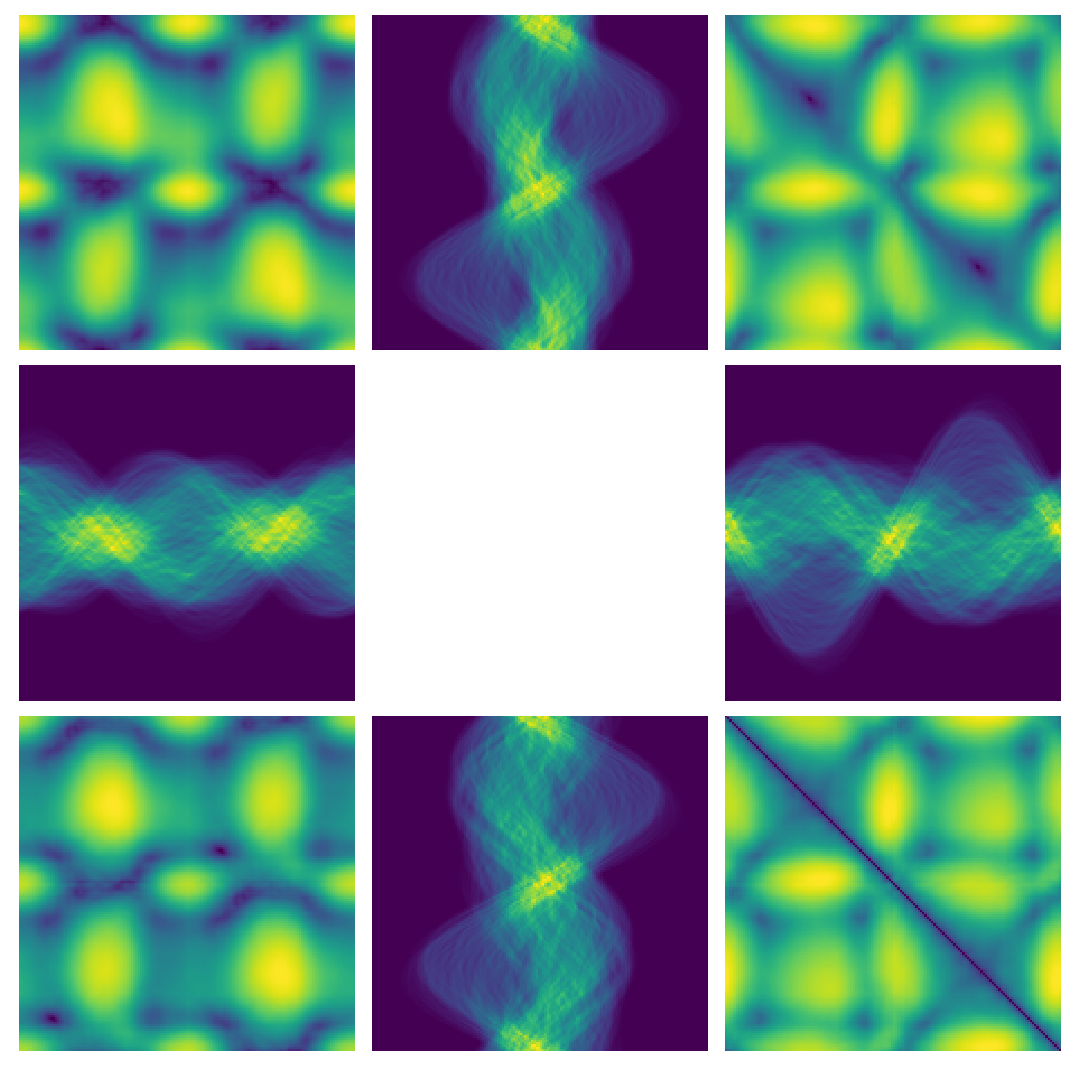
\includegraphics[width=0.45\textwidth]{images/Sinogram_3_comp.png}
%% \end{center}

% absolute position
%% \placetextbox[north west]{0.37}{0.33}{\setlength{\fboxsep}{0pt}\setlength{\fboxrule}{0.5pt}\fbox{absolute position1}}
%% \placetextbox[north west]{0.77}{0.33}{\setlength{\fboxsep}{0pt}\setlength{\fboxrule}{0.5pt}\fbox{absolute postion 2}}

% movie
%% \placetextbox[north west]{0.083}{0.30}{\movie[width=3.5cm,height=2cm,poster, externalviewer, loop]{\includegraphics[width=3.5cm]{movie_still.png}}{movie.webm}}
%%%%%%%%%%%%%%%%%%%%%%%%%%%%%%%%%%%%%%%%%%%%%%%%%%%%%%%%%%%%

%%%%%%%%%%%%%%%%%%%%%%%%%%%%%%%%%%%%%%%%%%%%%%%%%%%%%%%%%%%%
% absolute positioning of typeset material    
%%%%%%%%%%%%%%%%%%%%%%%%%%%%%%%%%%%%%%%%%%%%%%%%%%%%%%%%%%%%
\newcommand{\placetextbox}[4][center]{%
  % [#1]: box anchor: center (default) | 
  %                 south west | west | north west | north |
  %                 north east | east | south east | south | 
  %                 mid west | mid | mid east |
  %                 base west | base | base east 
  % #2: horizontal position (fraction of page width)
  % #3: vertical position (fraction of page height)
  % #4: content
  %
  \tikz[remember picture,overlay,x=\paperwidth,y=\paperheight]{%
    \node[anchor=#1,inner sep=0pt]
    at ($(current page.south west)+(#2,#3)$) {#4};
  }%
}
%%%%%%%%%%%%%%%%%%%%%%%%%%%%%%%%%%%%%%%%%%%%%%%%%%%%%%%%%%%%

\usetheme{Berlin}

% \usecolortheme[named=UBCblue]{structure}
% \usecolortheme[named=Mahogany]{structure} % Sample dvipsnames color
\definecolor{UBCblue}{rgb}{0.04706, 0.13725, 0.26667} % UBC Blue (primary)
\definecolor{UBCgrey}{rgb}{0.3686, 0.5255, 0.6235} % UBC Grey (secondary)

\definecolor{CLICbrown}{rgb}{0.438, 0.309, 0.313}
\definecolor{CLICorange}{rgb}{0.938, 0.660, 0.473}
\definecolor{CLICyellow}{rgb}{0.973, 0.938, 0.684}
\definecolor{CLICbg}{rgb}{0.113, 0.125, 0.129}
\definecolor{CLICfg}{rgb}{0.895, 0.895, 0.895}

%% \setbeamercolor{palette primary}{bg=CLICbrown,fg=white}
%% \setbeamercolor{palette secondary}{bg=CLICorange,fg=white}
%% \setbeamercolor{palette tertiary}{bg=CLICyellow,fg=white}
%% % \setbeamercolor{palette quaternary}{bg=CLICbrown,fg=white}
\setbeamercolor{structure}{fg=CLICbg} % itemize, enumerate, etc
\setbeamercolor{structure}{bg=CLICbg} % itemize, enumerate, etc
\setbeamercolor{section in toc}{fg=CLICbg} % TOC sections

%% % Override palette coloring with secondary
% \setbeamercolor{subsection in head/foot}{bg=UBCgrey,fg=white}
%% \setbeamercolor{normal text}{bg=CLICfg, fg=CLICfg}
%% \setbeamercolor{background canvas}{bg=CLICbg}


\def\liketitle#1{%
{\usebeamerfont{frametitle}\usebeamercolor[fg]{structure}%
\begin{flushleft}%
\vspace{-\baselineskip}% Cometic correction for space introduced by flushleft
#1\par
\end{flushleft}%
\vspace{-\baselineskip}% Cosmetic correction for space introduced by flushleft
}%
\vspace{0.75\baselineskip}%
}
\subtitle{
\includegraphics[width=4cm]{images/logo_transparent.png}\\Common Lines Implied Clustering}
\author{Donovan Webb}
\institute{eBIC/University of Bath}
\date{}
\titlegraphic{
\includegraphics[width=3cm]{images/Diamond.png}}

\AtBeginSection[]{
  \begin{frame}
  \vfill
  \centering
  \begin{beamercolorbox}[sep=8pt,center,shadow=false,rounded=false]{title}
    \usebeamerfont{title}\insertsectionhead\par%
  \end{beamercolorbox}
  \vfill
  \end{frame}
}

\addtobeamertemplate{frametitle}{}{%
\begin{textblock*}{100mm}(.88\textwidth,-1cm)

\includegraphics[width=2cm, keepaspectratio]{images/logo_transparent.png}
\end{textblock*}}


\begin{document}

\setbeamertemplate{navigation symbols}{}
\begin{frame}[plain]
\setbeamercolor{title}{bg=white,fg=CLICbg}
  \maketitle
\setbeamercolor{title}{bg=CLICbg,fg=CLICfg}
\end{frame}
\addtocounter{framenumber}{-1} % Don't count title slide

%% \begin{frame}{Table of Contents}
%%   \tableofcontents[sectionstyle=show/show, hideallsubsections]
%% \end{frame}
%!XXXX Intro!

\section{Common Lines}

\begin{frame}[fragile]{A Shared Single Line}
 \begin{center}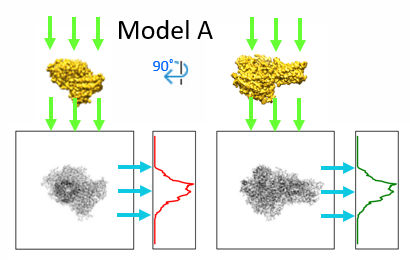
\includegraphics[width=0.6\textwidth]{images/lines_one_models.png}
    \end{center}
\end{frame}

\begin{frame}[fragile]{Common Lines}
  \textbf{Two projections of the same 3D volume share at least one common line in the Radon transform}
 \begin{center}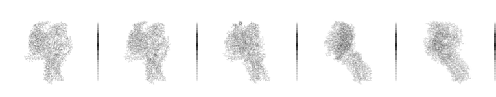
\includegraphics[width=0.85\textwidth]{images/common_line.png}
    \end{center}
 \begin{center}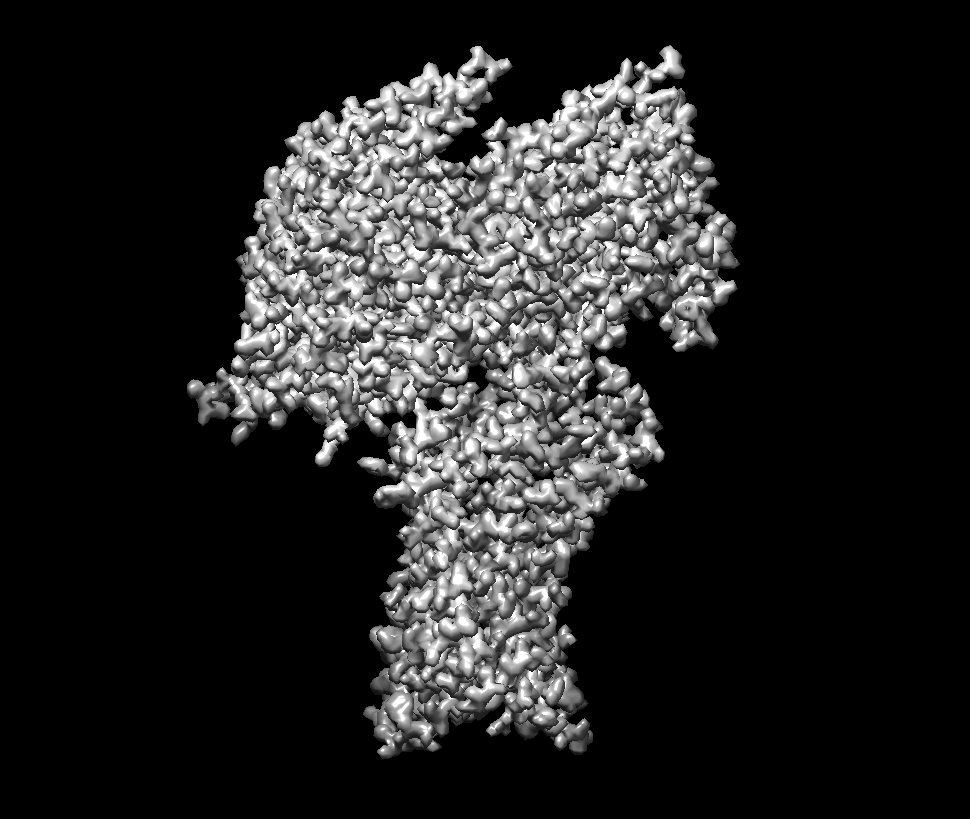
\includegraphics[width=0.35\textwidth]{images/3D_model.png}
    \end{center}
\end{frame}

%% \begin{frame}[fragile]{The Radon Transform}
%%  \begin{center}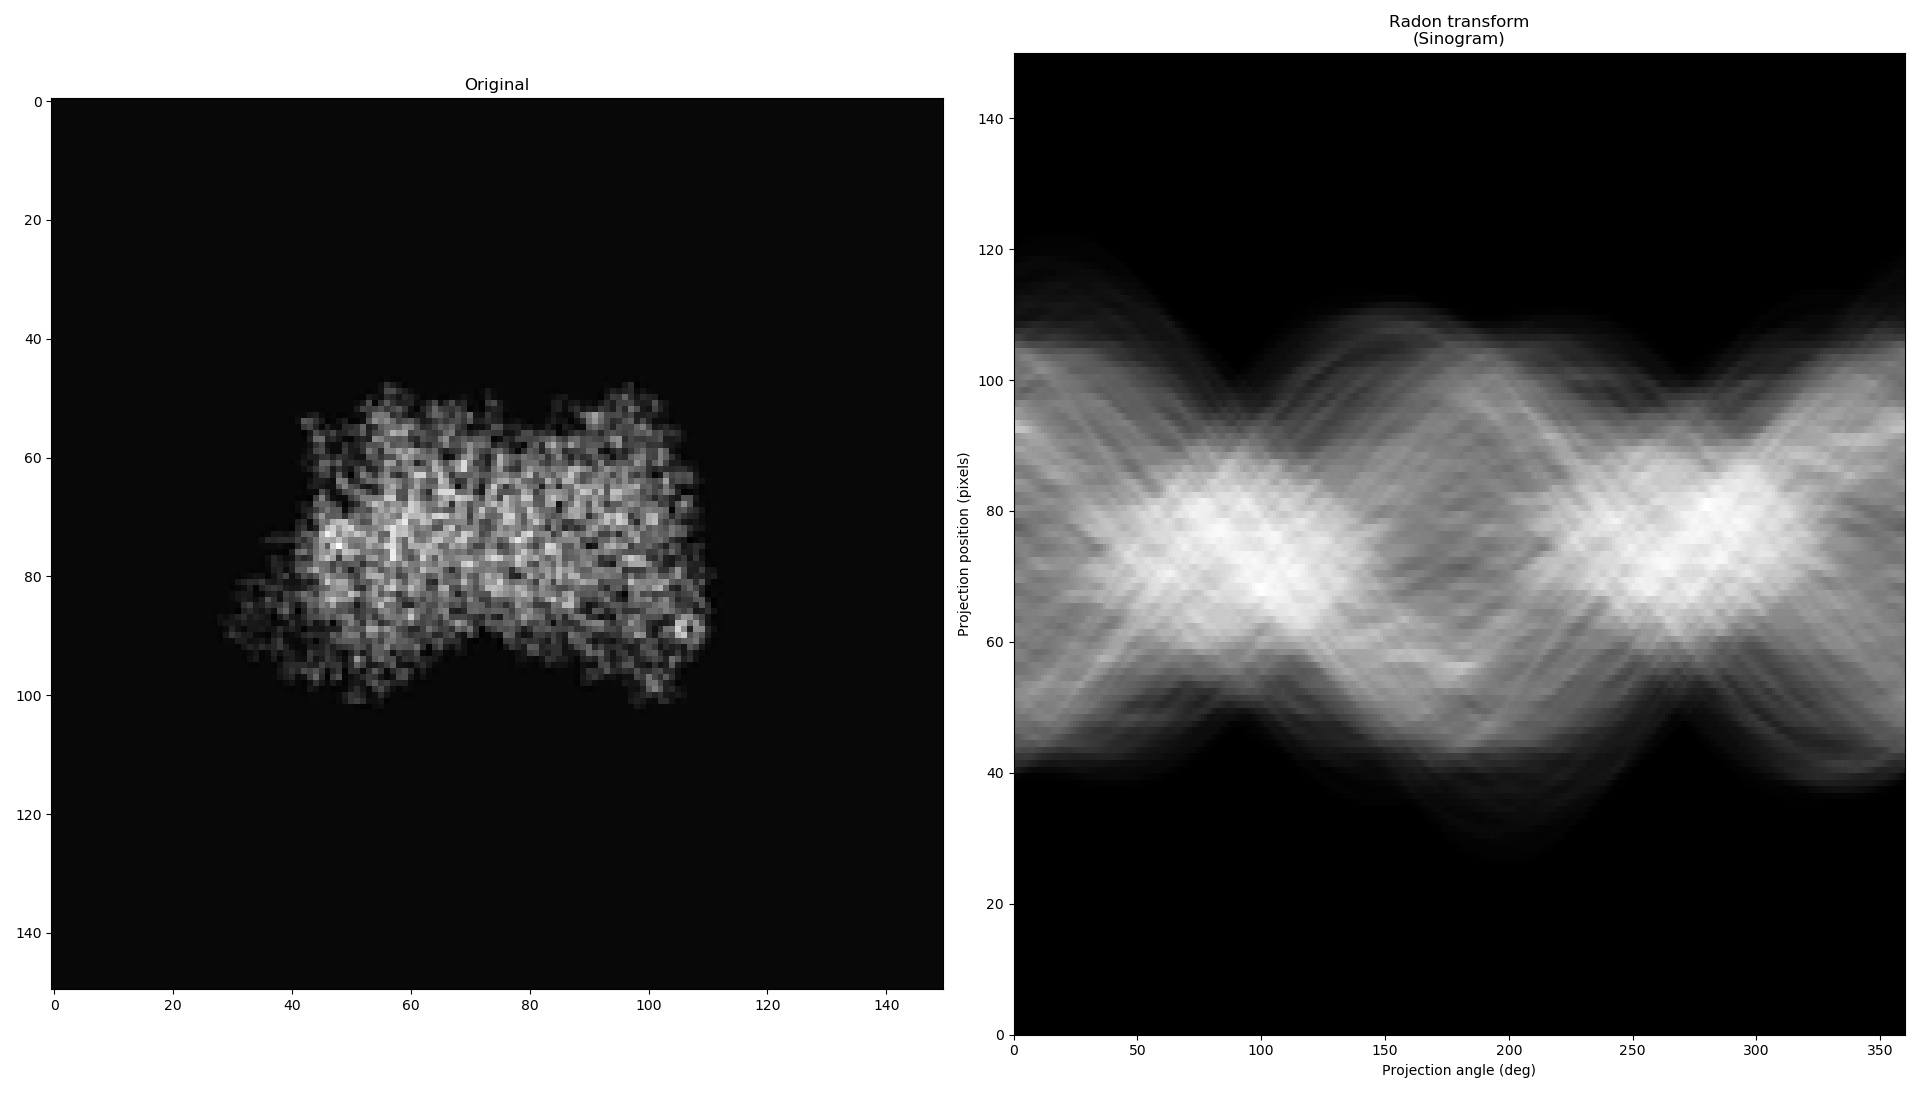
\includegraphics[width=0.9\textwidth]{images/Sinogram_Proj1.png}
%%     \end{center}
%% \vspace{-1em}
%% \end{frame}

\begin{frame}[fragile]{The Radon Transform}
 \only<1>{\begin{center}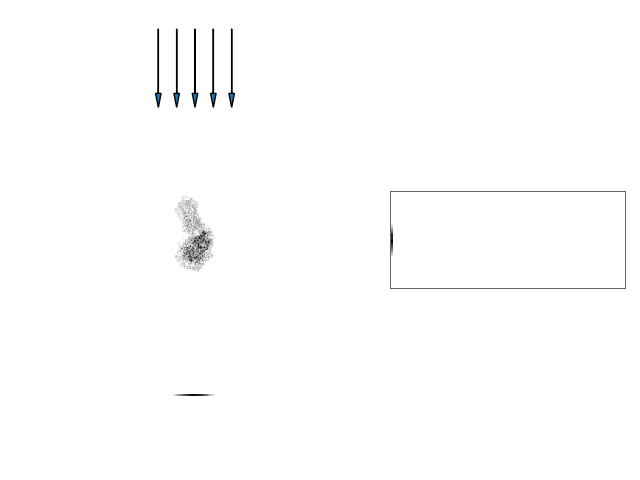
\includegraphics[width=0.85\textwidth]{images/sino_ani/sino_make_fr1.png}
    \end{center}}
 \only<2>{\begin{center}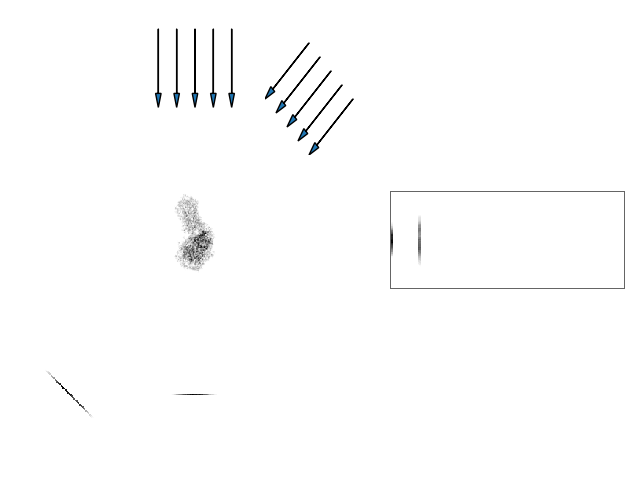
\includegraphics[width=0.85\textwidth]{images/sino_ani/sino_make_fr2.png}
    \end{center}}
 \only<3>{\begin{center}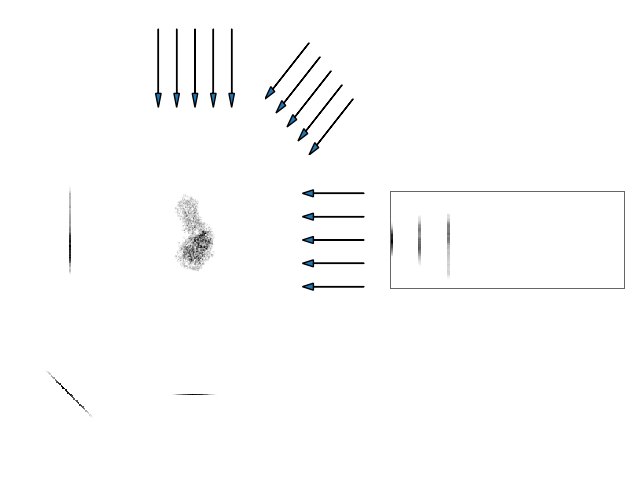
\includegraphics[width=0.85\textwidth]{images/sino_ani/sino_make_fr3.png}
    \end{center}}
 \only<4>{\begin{center}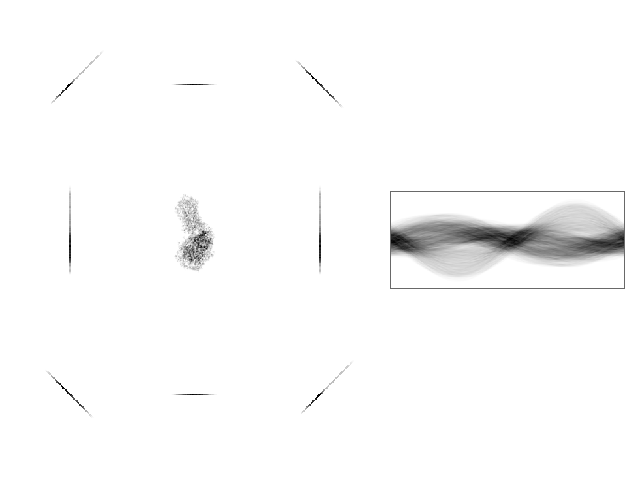
\includegraphics[width=0.85\textwidth]{images/sino_ani/sino_make_fr4.png}
    \end{center}}
\end{frame}

\begin{frame}{The Problem}
  \textbf{Can projections of different models be separated based on similarities and differences between common lines?}
  \begin{center}
    \begin{minipage}{0.45\textwidth}
      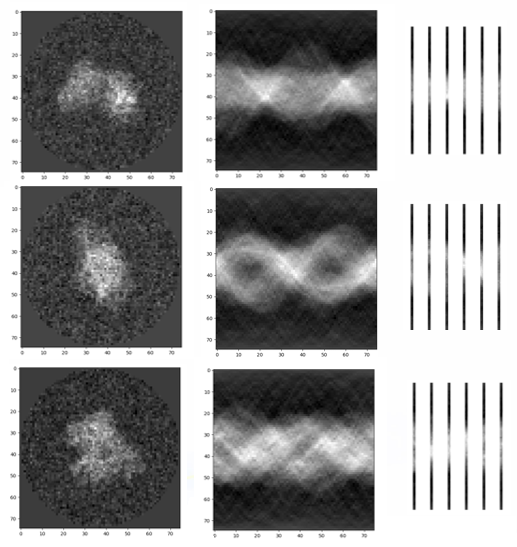
\includegraphics[width=0.9\textwidth]{images/proj_sin_lin.png}
    \end{minipage}
    ~
    \begin{minipage}{0.45\textwidth}
      \begin{center}
        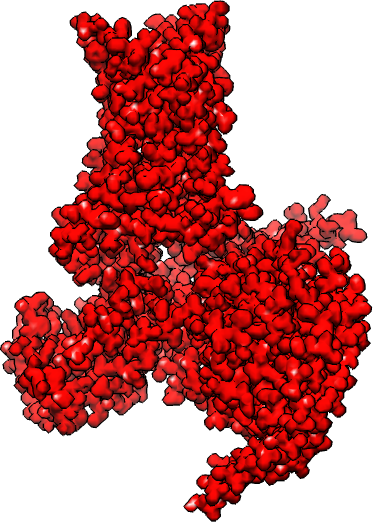
\includegraphics[height=0.4\textheight]{images/figures/no_e.png}
        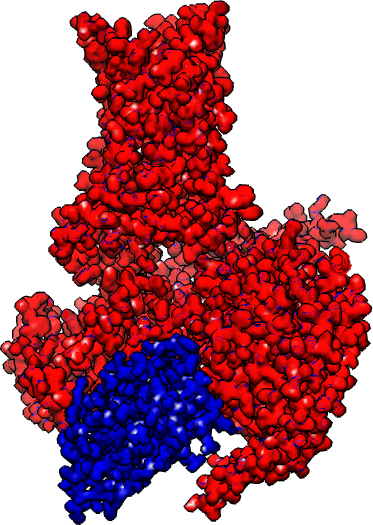
\includegraphics[height=0.4\textheight]{images/figures/all_edit.png}
      \end{center}
    \end{minipage}
  \end{center}
\end{frame}

\begin{frame}[fragile]{Common Lines Between Different Models}
  \centering\textbf{What about two different 3D volumes?}
 \begin{center}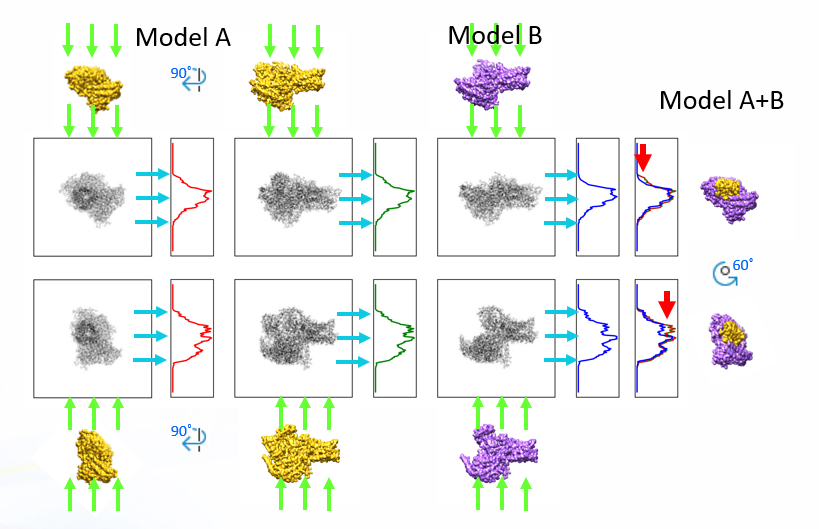
\includegraphics[width=0.85\textwidth]{images/lines_two_models.png}
    \end{center}
\end{frame}

\section{Finding Common Lines}

\begin{frame}[fragile]{Sinogram Cross Correlation}
  \centering\textbf{Finding the common line between two sinograms}
  \only<1>
    {\begin{center}
      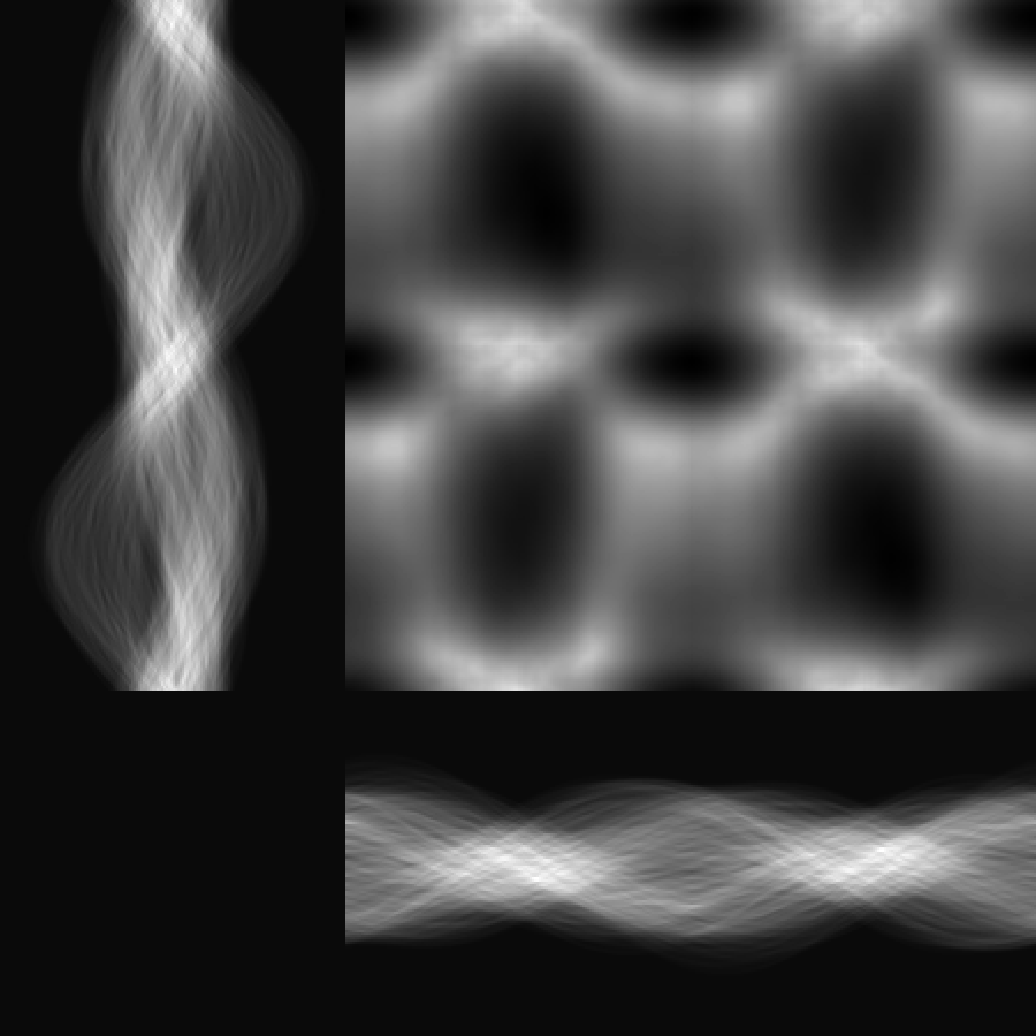
\includegraphics[width=0.4\textwidth]{images/2sin_comp.png}
      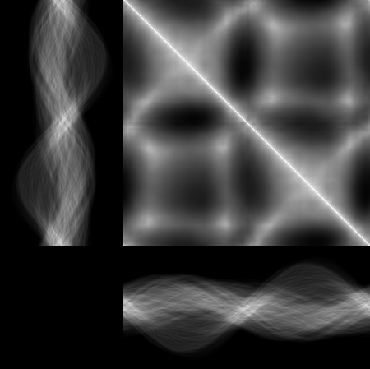
\includegraphics[width=0.4\textwidth]{images/self_correl.png}
    \end{center}}
  \only<2,3,4>{
    \begin{center}
      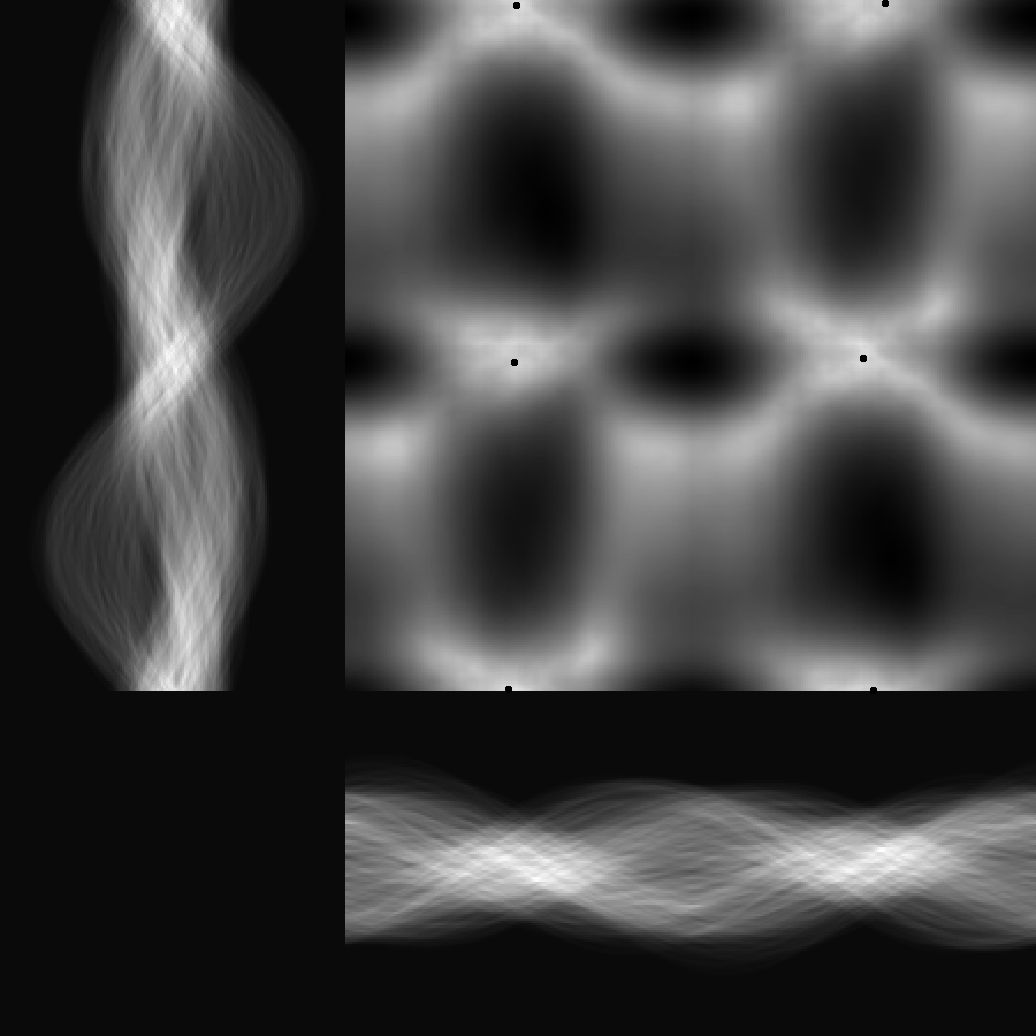
\includegraphics[width=0.4\textwidth]{images/2sin_comp_peaks.png}
      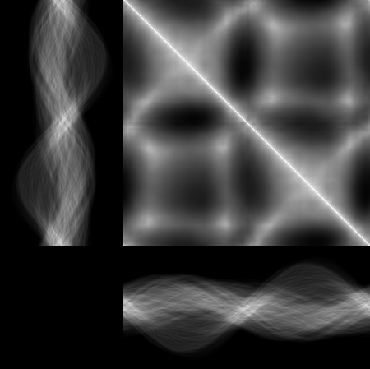
\includegraphics[width=0.4\textwidth]{images/self_correl.png}
    \end{center}}
  \pause
  \pause
  \centering\textbf{But what about N sinograms?} \\
  \pause
  \centering\textbf{What about N sinograms from a heterogenous dataset?}

\end{frame}


\begin{frame}[fragile]{Concept's flowchart}
  \begin{center}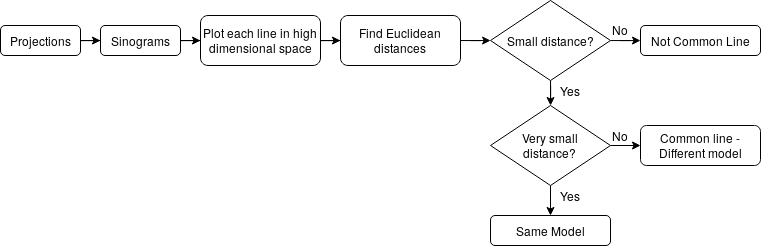
\includegraphics[width=1\textwidth]{images/first_pipeline.png}
    \end{center}
  
    \placetextbox[north west]{0.05}{0.60}{\setlength{\fboxsep}{0pt}\setlength{\fboxrule}{0.5pt}\begin{minipage}{0.6\textwidth}
      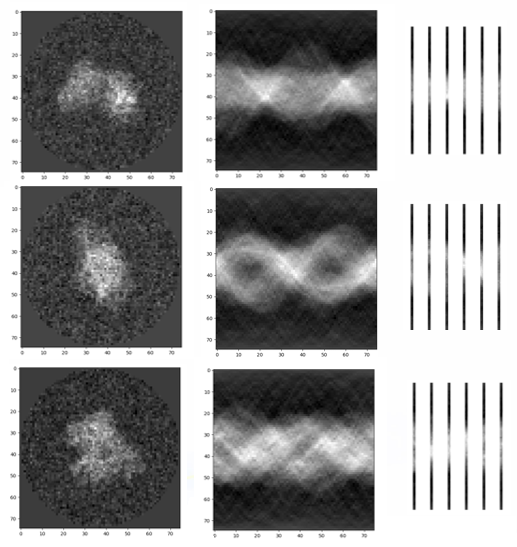
\includegraphics[width=0.3\textwidth]{images/proj_sin_lin.png}
      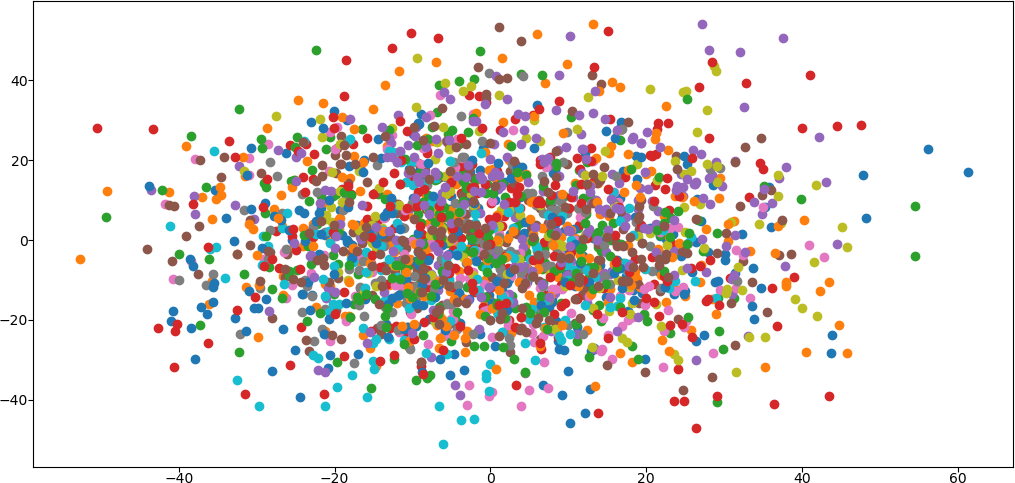
\includegraphics[width=0.65\textwidth]{images/no_dimred.png} 
      \small{15 projections - 2 models - 75 dimensional space}
      \end{minipage}
    }

    \vspace{1em}
    \pause
    Curse of Dimensionality.
\end{frame}

\section{Dimensional Reduction}

\begin{frame}[fragile]{Dimensional Reduction - Linear (PCA)}
  \textbf{How to display high dimensional data in lower dimensional space?}
  \begin{center}
  \only<1>{\hspace{0.35em}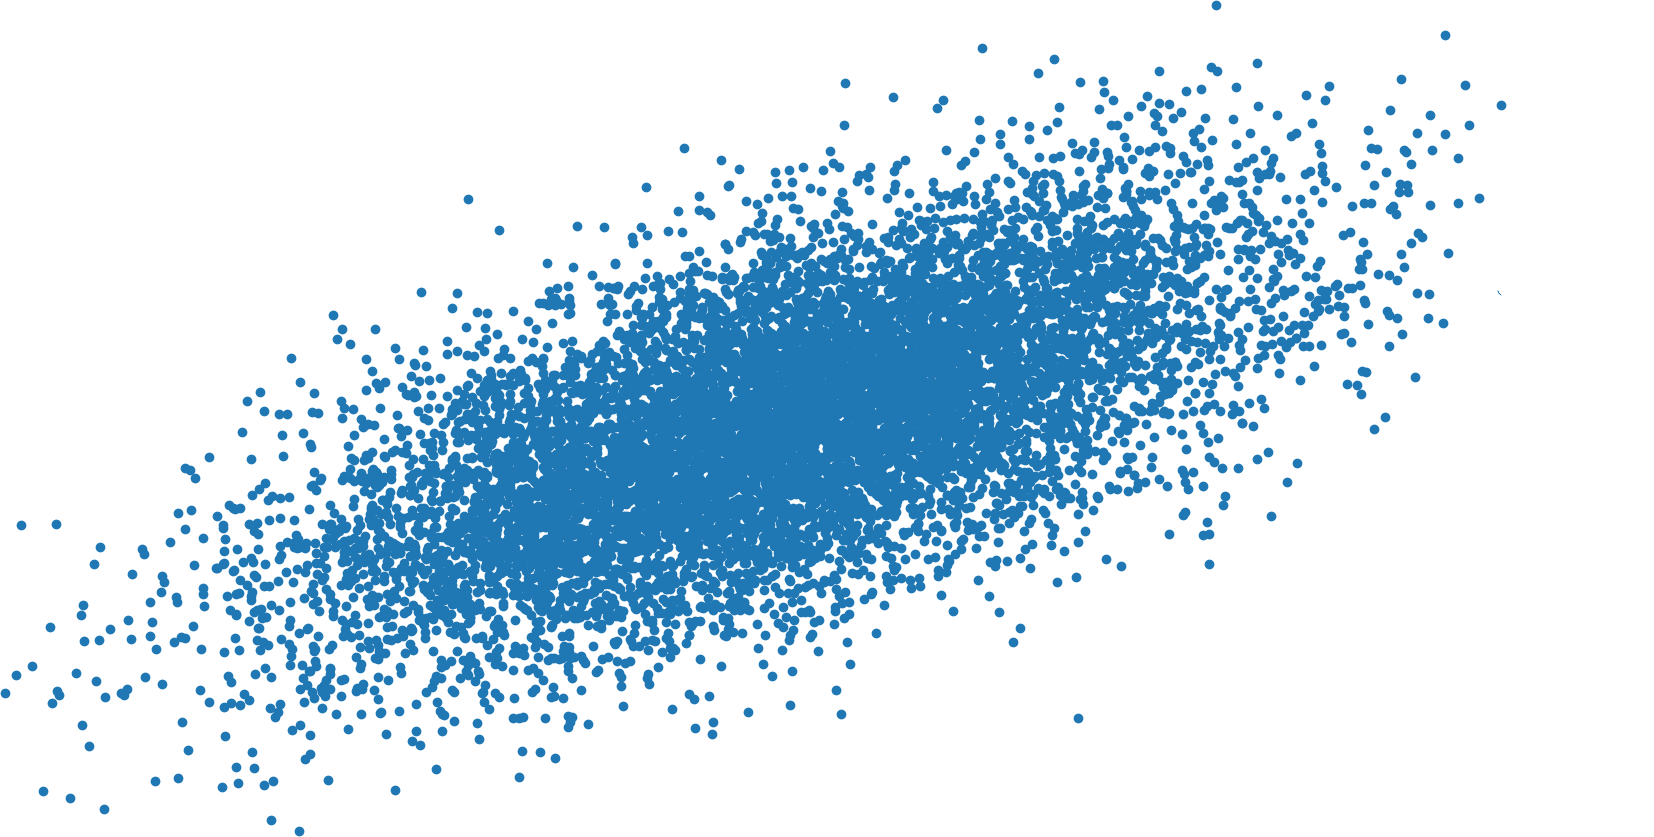
\includegraphics[width=0.7\textwidth]{images/pcavsmani/PCA2D.png}}
  \only<2>{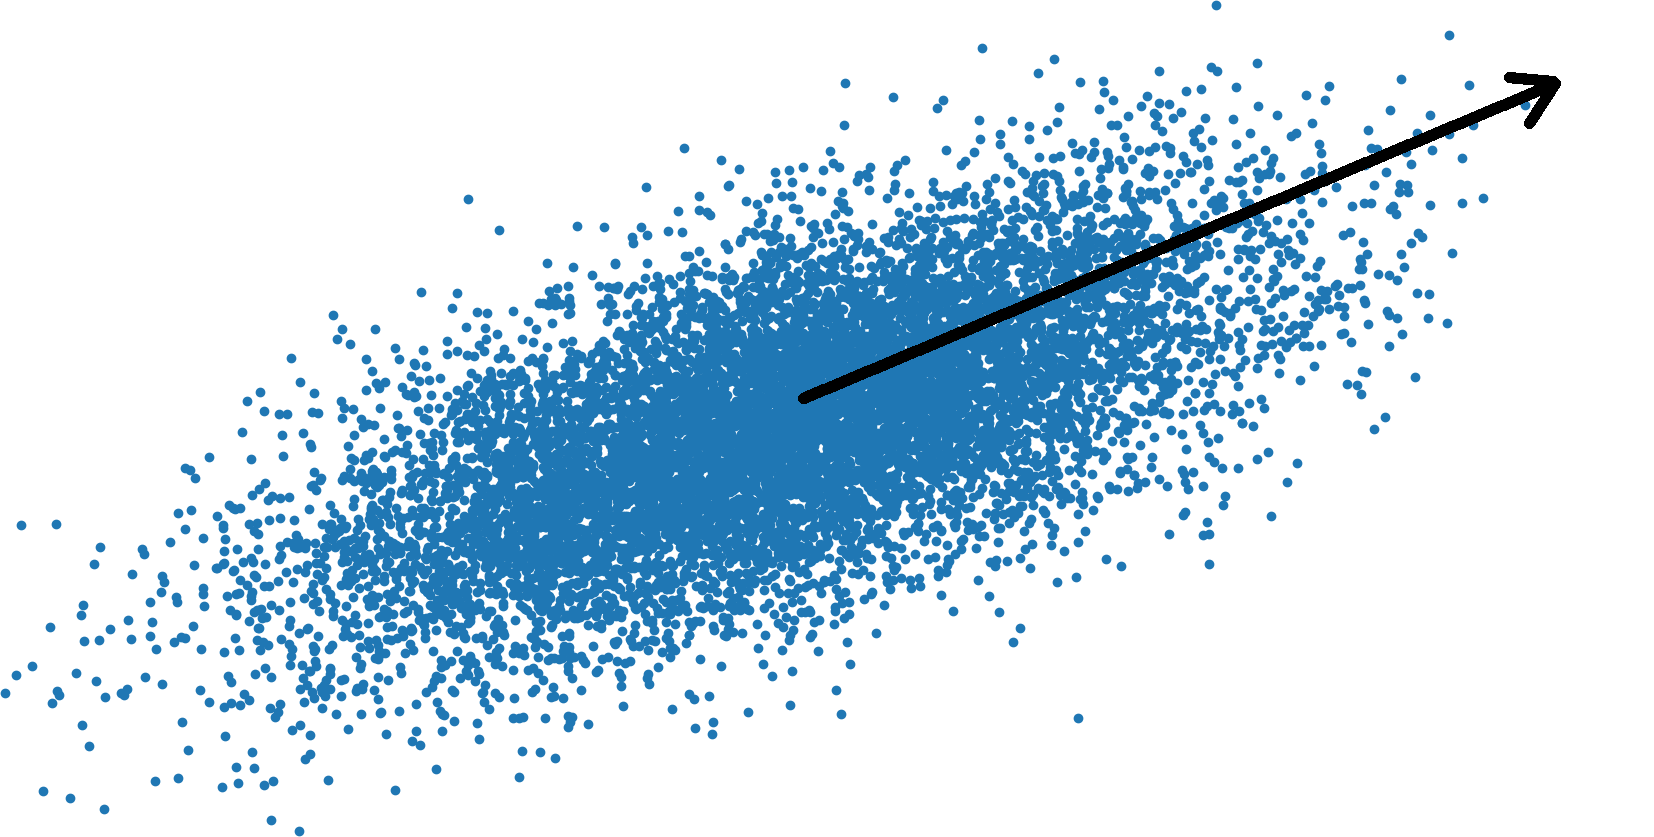
\includegraphics[width=0.7\textwidth]{images/pcavsmani/PCA2D1comp.png}}
  \only<3>{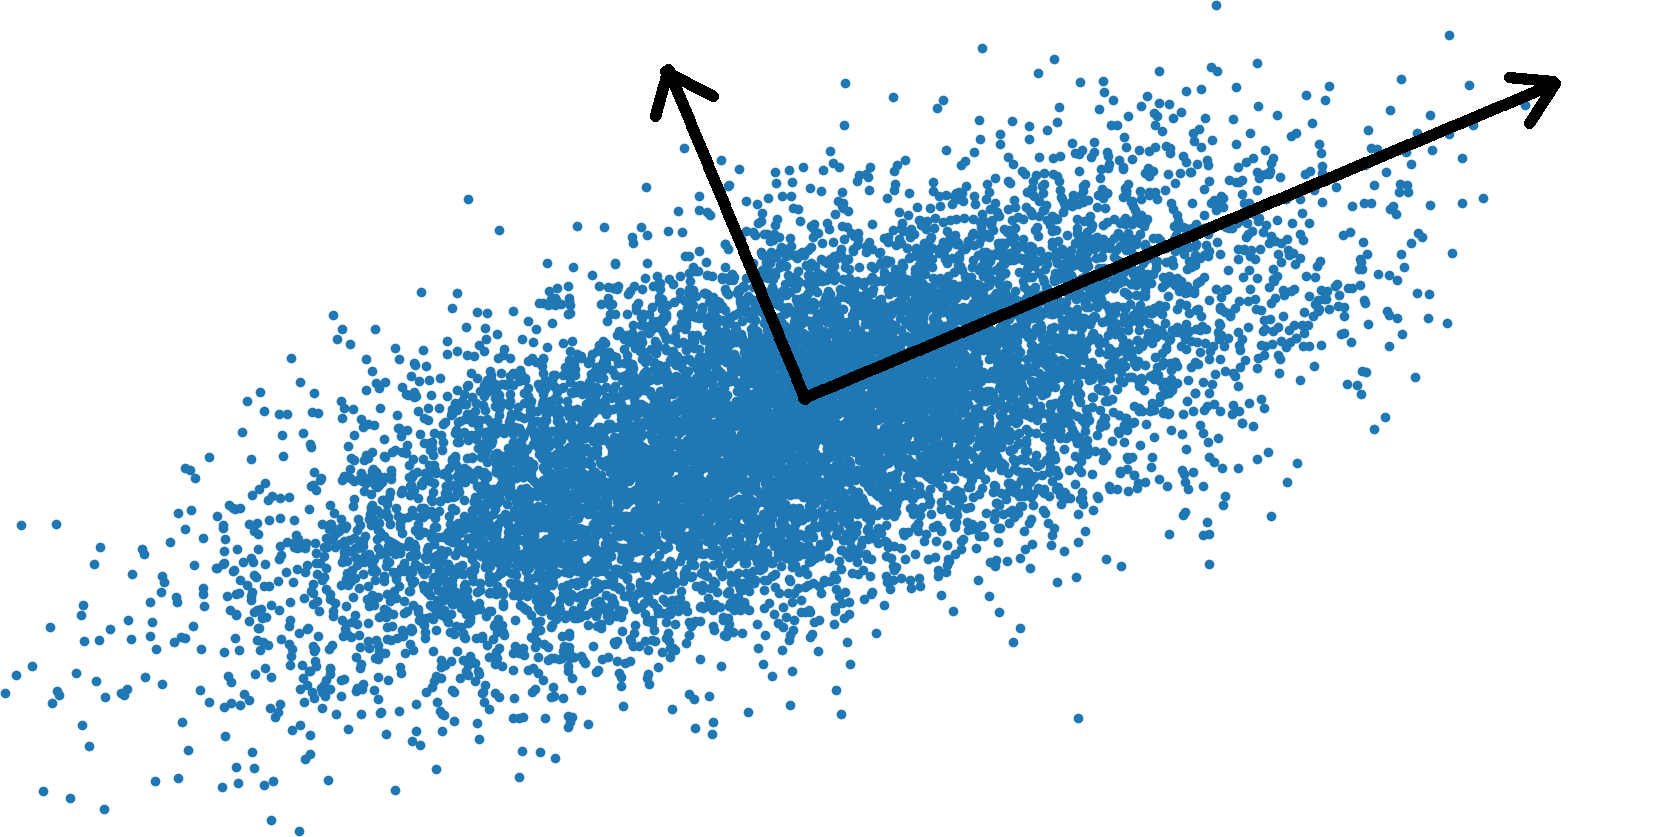
\includegraphics[width=0.7\textwidth]{images/pcavsmani/PCA2D2comp.png}}
  \end{center}
\end{frame}

\begin{frame}[fragile]{Linear vs Non-Linear - Swiss Roll} 
                  \vspace{-1em}
	\begin{center}
		  \fbox{\begin{minipage}[t][0.3\textheight][t]{0.45\textwidth}
                    \begin{center} 
                    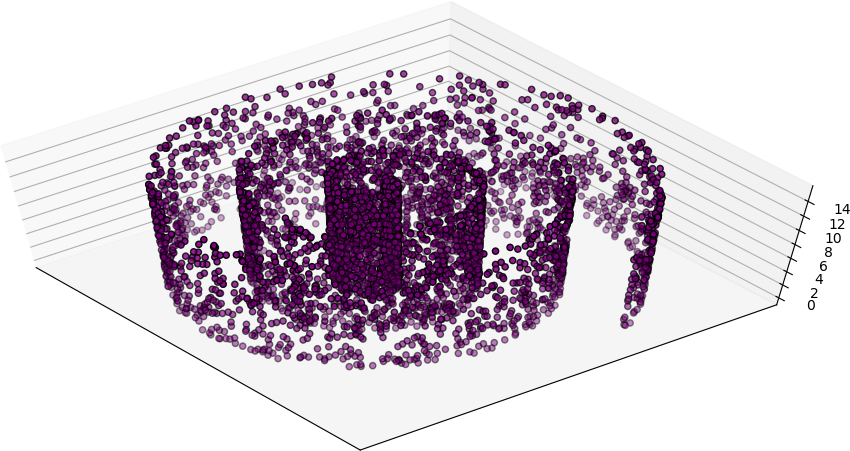
\includegraphics[width=0.45\textwidth]{images/pcavsmani/swiss_blank_1_crop.png}
                    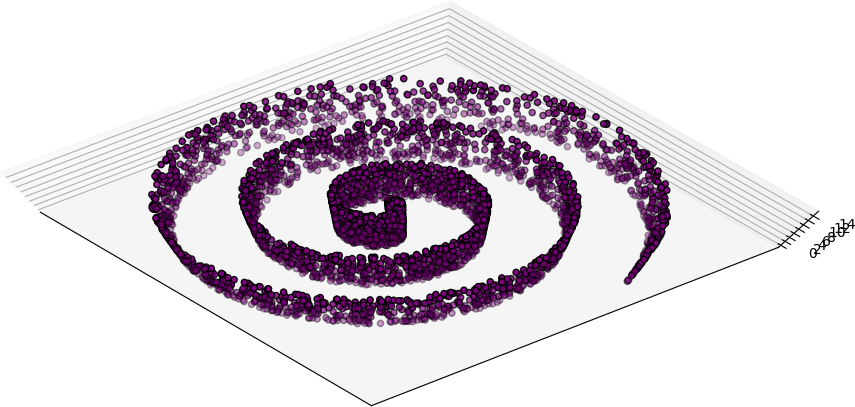
\includegraphics[width=0.45\textwidth]{images/pcavsmani/swiss_blank_2_crop.png}
                    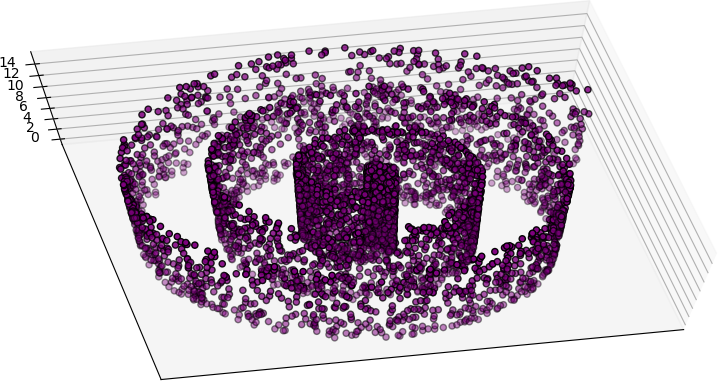
\includegraphics[width=0.45\textwidth]{images/pcavsmani/swiss_blank_3_crop.png}
                    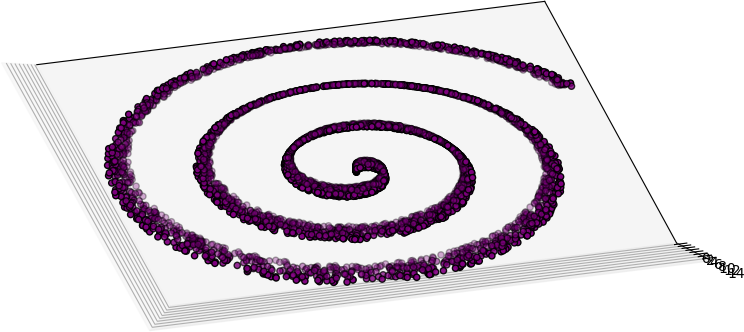
\includegraphics[width=0.45\textwidth]{images/pcavsmani/swiss_blank_4_crop.png}
                    \end{center}
		  \end{minipage}}
                  %\hspace{1em}
		  \fbox{\begin{minipage}[t][0.4\textheight][t]{0.45\textwidth}
                    \begin{center}
                    \only<1>{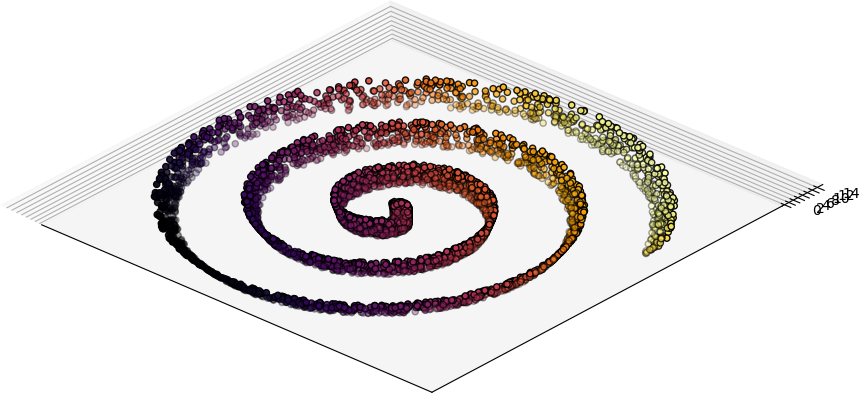
\includegraphics[width=0.65\textwidth]{images/pcavsmani/swiss_PCA_2_crop.png} \\}
                    \only<2,3>{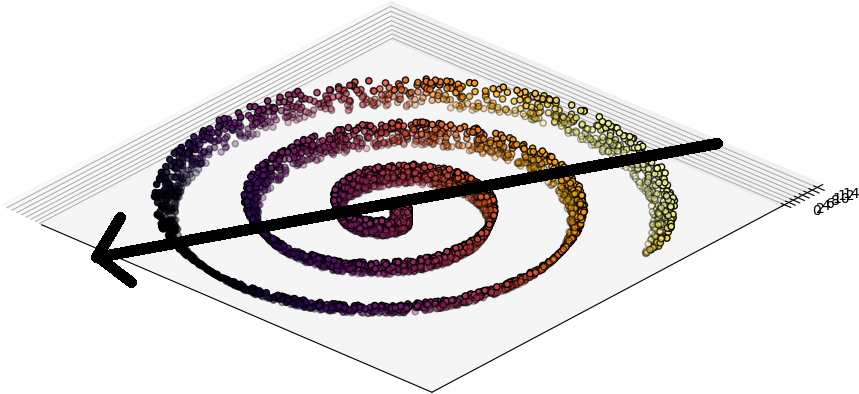
\includegraphics[width=0.65\textwidth]{images/pcavsmani/swiss_PCA_2_crop_arrow.png} \\}
                    \only<1>{PCA \\
                    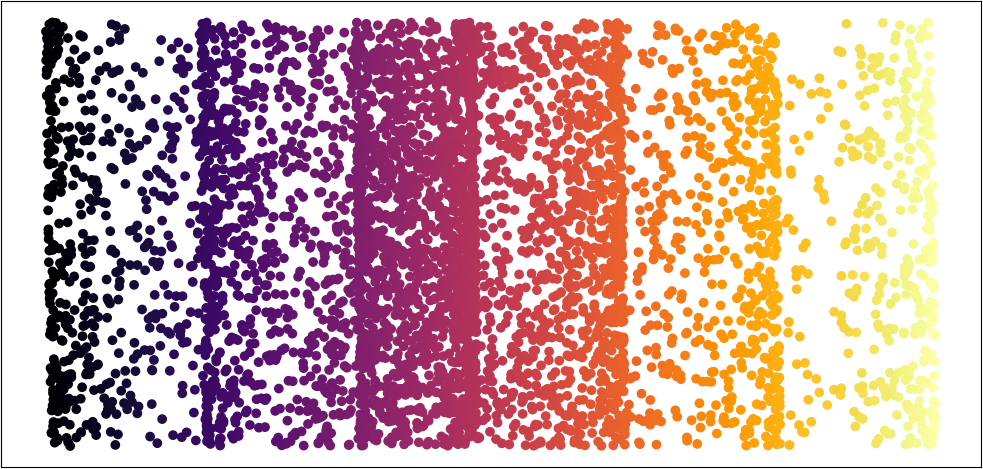
\includegraphics[width=0.45\textwidth]{images/pcavsmani/swiss_pca_2D_crop.png}
                    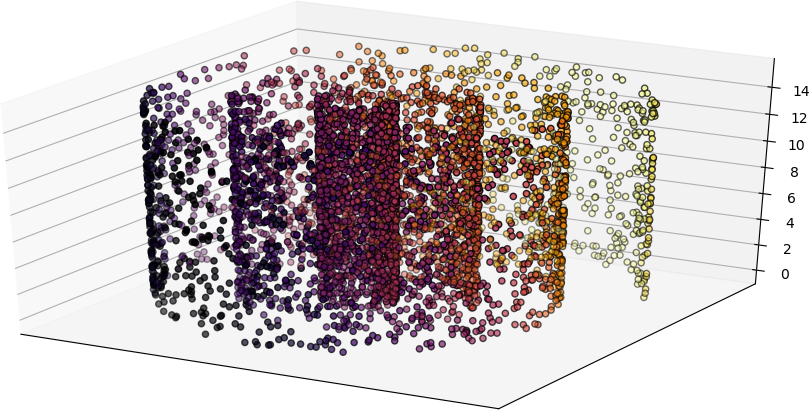
\includegraphics[width=0.45\textwidth]{images/pcavsmani/swiss_PCA_1_crop.png}}
                    \only<2,3>{PCA \\
                    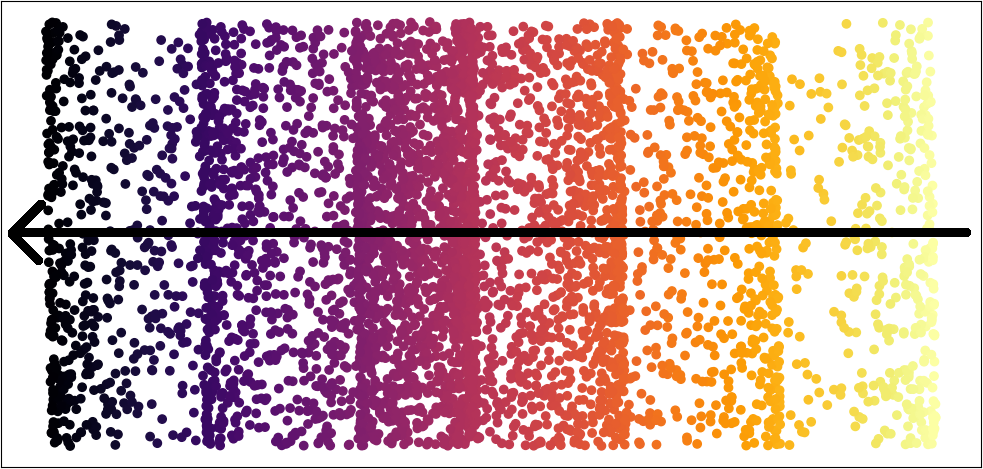
\includegraphics[width=0.45\textwidth]{images/pcavsmani/swiss_pca_2D_crop_arrow.png}
                    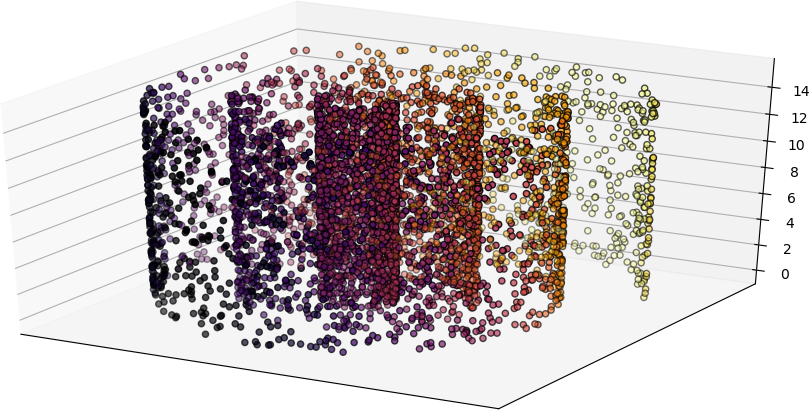
\includegraphics[width=0.45\textwidth]{images/pcavsmani/swiss_PCA_1_crop.png}}
                    \end{center}
		  \end{minipage}}
                  ~
		  \fbox{\begin{minipage}[t][0.40\textheight][t]{0.45\textwidth}
                    \begin{center}
                    \only<1,2>{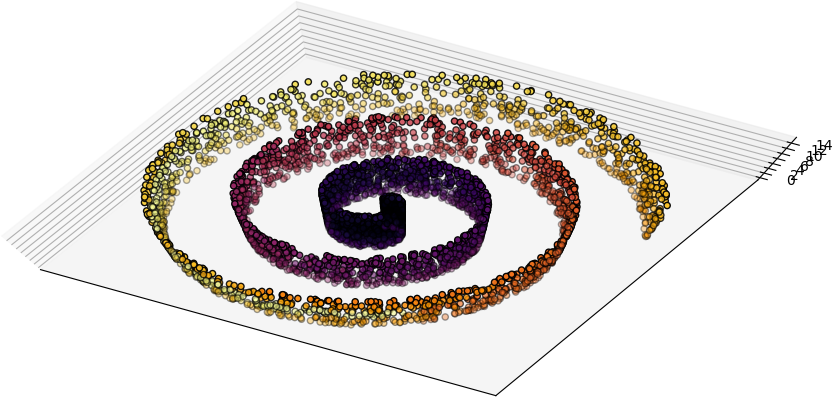
\includegraphics[width=0.65\textwidth]{images/pcavsmani/swiss_UMAP_2_crop.png}\\}
                    \only<3>{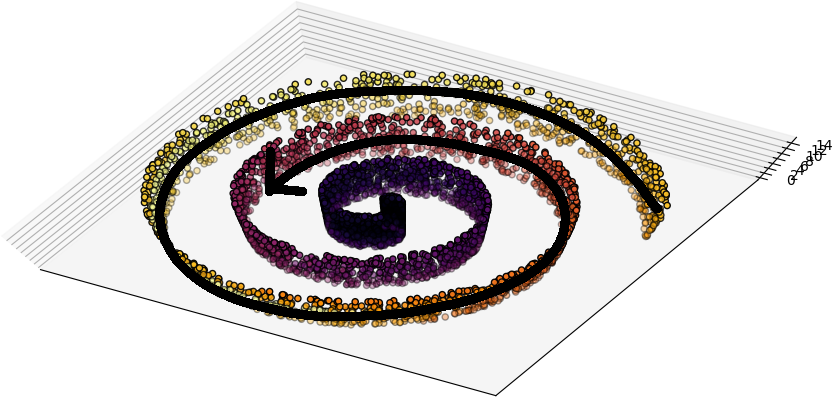
\includegraphics[width=0.65\textwidth]{images/pcavsmani/swiss_UMAP_2_crop_arrow.png}\\}
                    \only<1,2>{UMAP \\
                    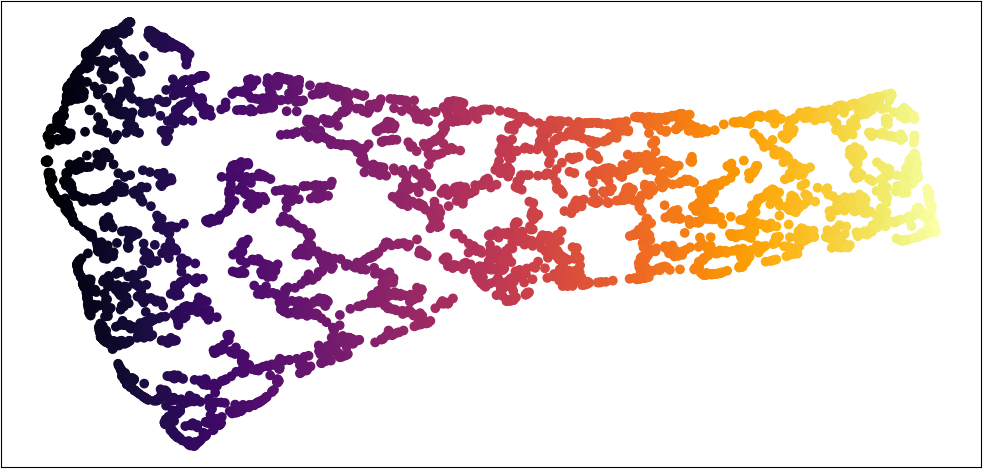
\includegraphics[width=0.45\textwidth]{images/pcavsmani/swiss_UMAP_2D_crop.png}
                    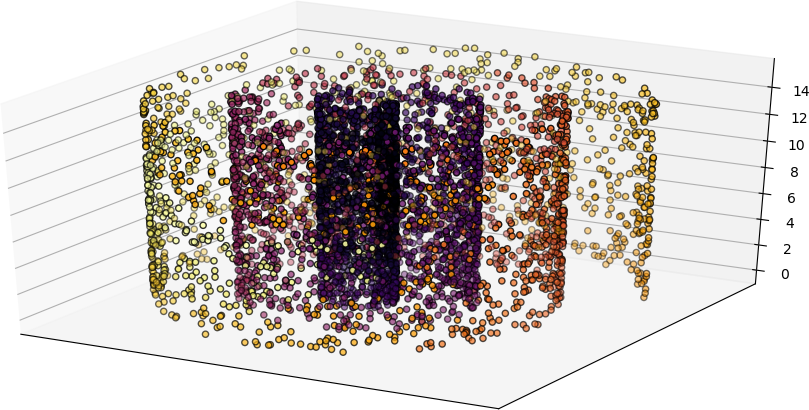
\includegraphics[width=0.45\textwidth]{images/pcavsmani/swiss_UMAP_1_crop.png}}
                    \only<3>{UMAP \\
                    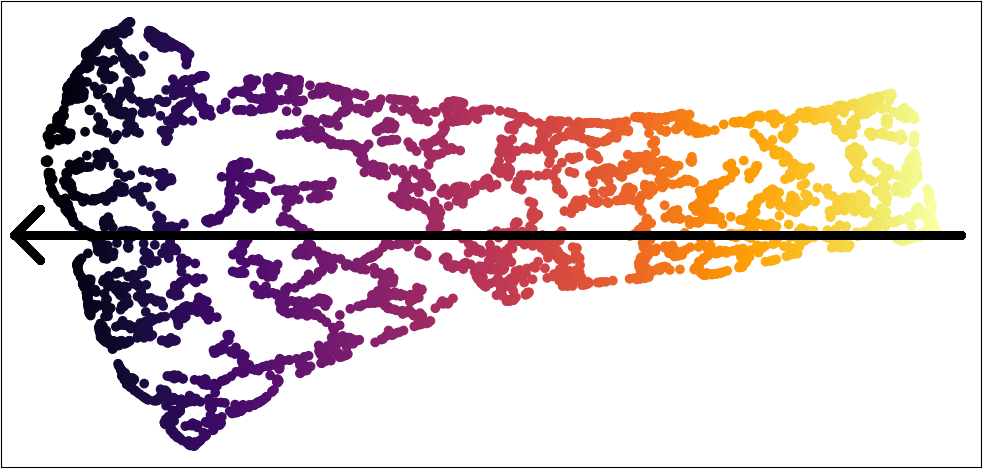
\includegraphics[width=0.45\textwidth]{images/pcavsmani/swiss_UMAP_2D_crop_arrow.png}
                    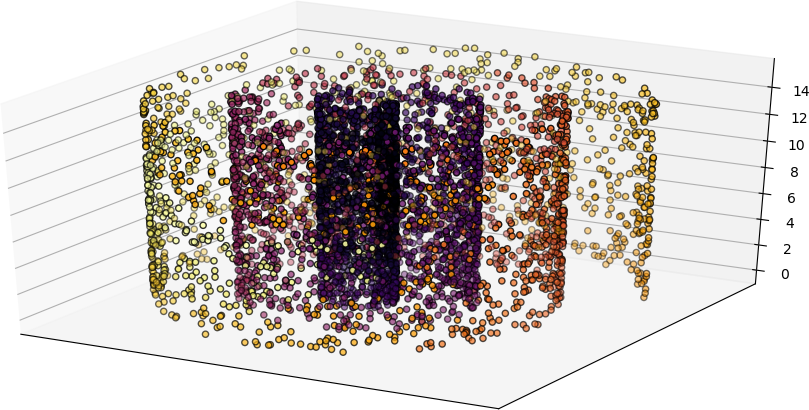
\includegraphics[width=0.45\textwidth]{images/pcavsmani/swiss_UMAP_1_crop.png}}
                    \end{center}
		  \end{minipage}}
                  ~
		  \begin{minipage}[t][0.3\textheight][t]{0.45\textwidth}
                    UMAP finds manifold, PCA does not
		  \end{minipage}
	\end{center}
\end{frame}

\begin{frame}[fragile]{Dimensional Reduction - Linear}
  % Dimensional reduction can be used to lower influence of noise and try to find common features of data.
  % Manifold learning found to improve accuracy of common lines being chosen although more computationally expensive.
  \only<1>{
  \vspace{-1em}\begin{center}
    \textbf{Find features - Reduce noise} \\
    \textbf{Linear} (PCA) \\
    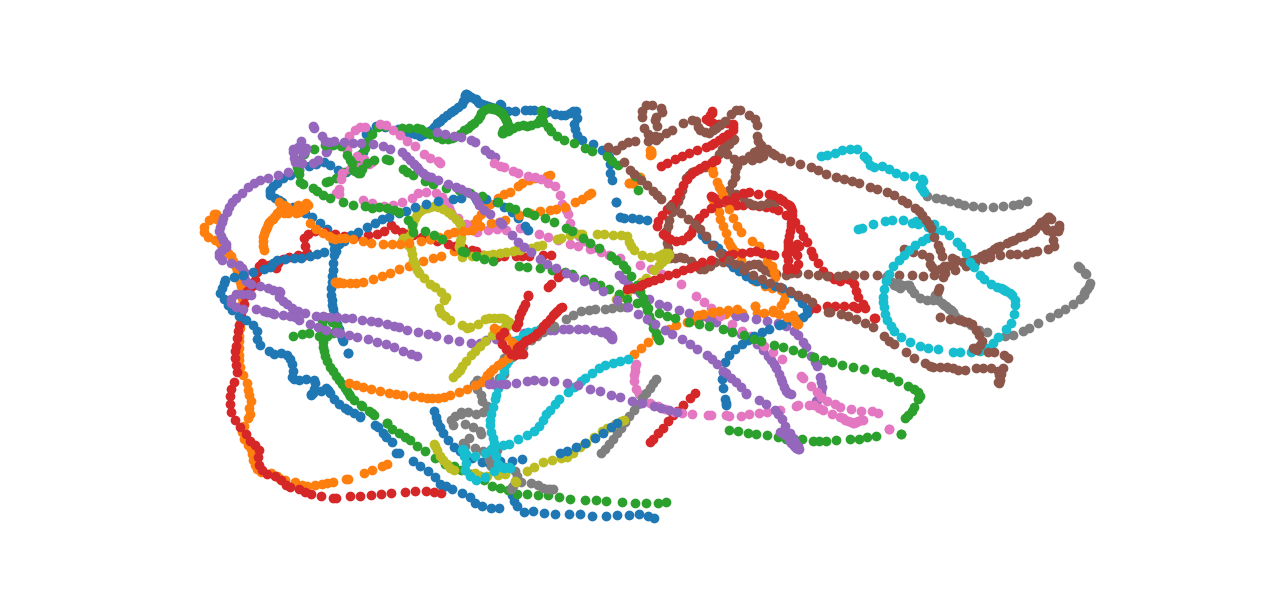
\includegraphics[width=0.8\textwidth]{images/dimredcomps/PCA_sins.png}
  \end{center}}

  \only<2>{
  \vspace{-1em}\begin{center}
    \textbf{Find features - Reduce noise} \\
    \textbf{Linear} (PCA) \\
    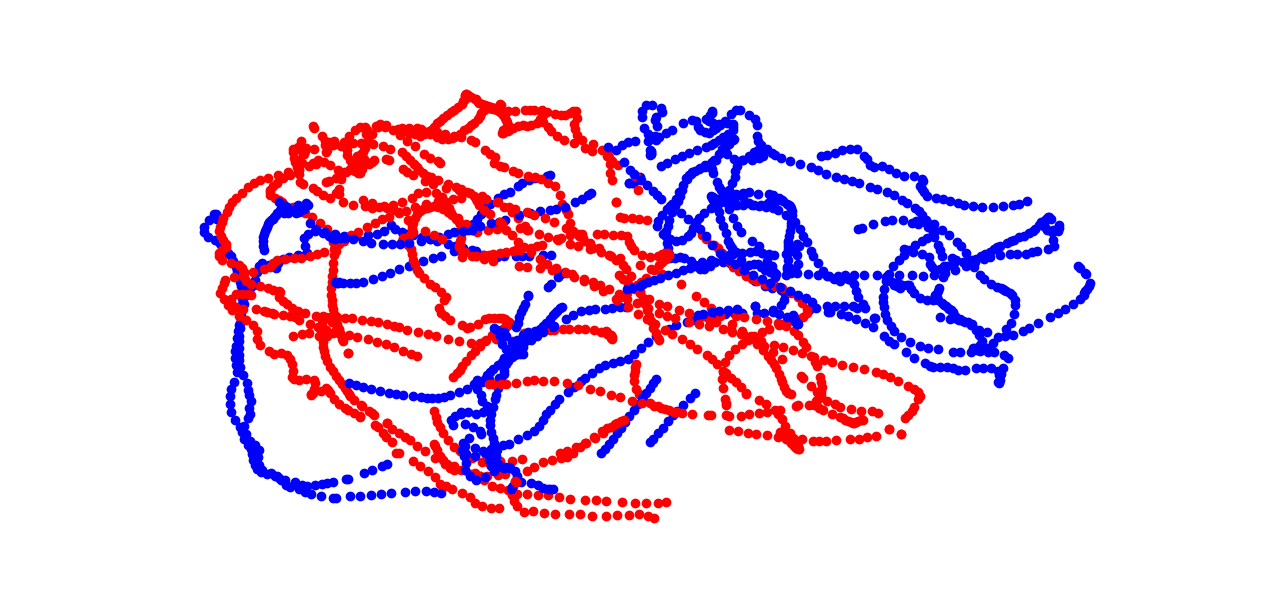
\includegraphics[width=0.8\textwidth]{images/dimredcomps/PCA_gt.png}
  \end{center}
 \placetextbox[north west]{0.04}{0.62}{\setlength{\fboxsep}{0pt}\setlength{\fboxrule}{0.5pt}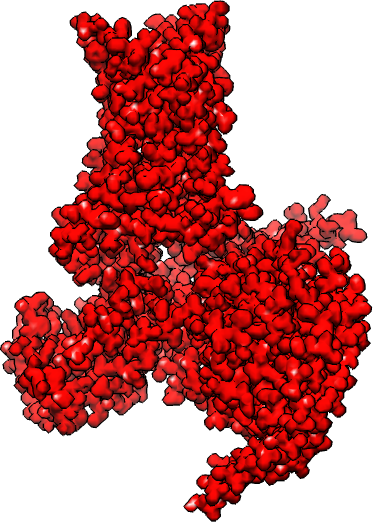
\includegraphics[width=0.25\textwidth]{images/figures/no_e.png}}
 \placetextbox[north west]{0.75}{0.62}{\setlength{\fboxsep}{0pt}\setlength{\fboxrule}{0.5pt}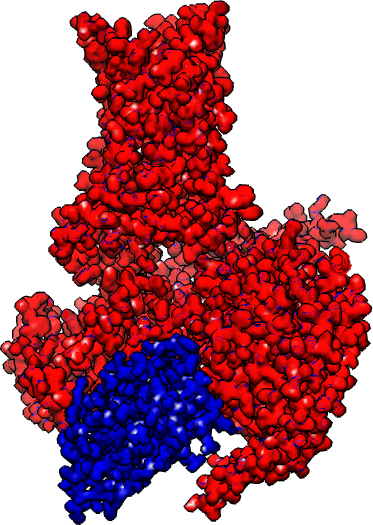
\includegraphics[width=0.25\textwidth]{images/figures/all_edit.png}}
  }
\end{frame}

\begin{frame}[fragile]{Dimensional Reduction - Non-Linear} 
	\only<1>{
	\begin{center}
		  \begin{minipage}{0.47\textwidth}
	          LLE\\
                  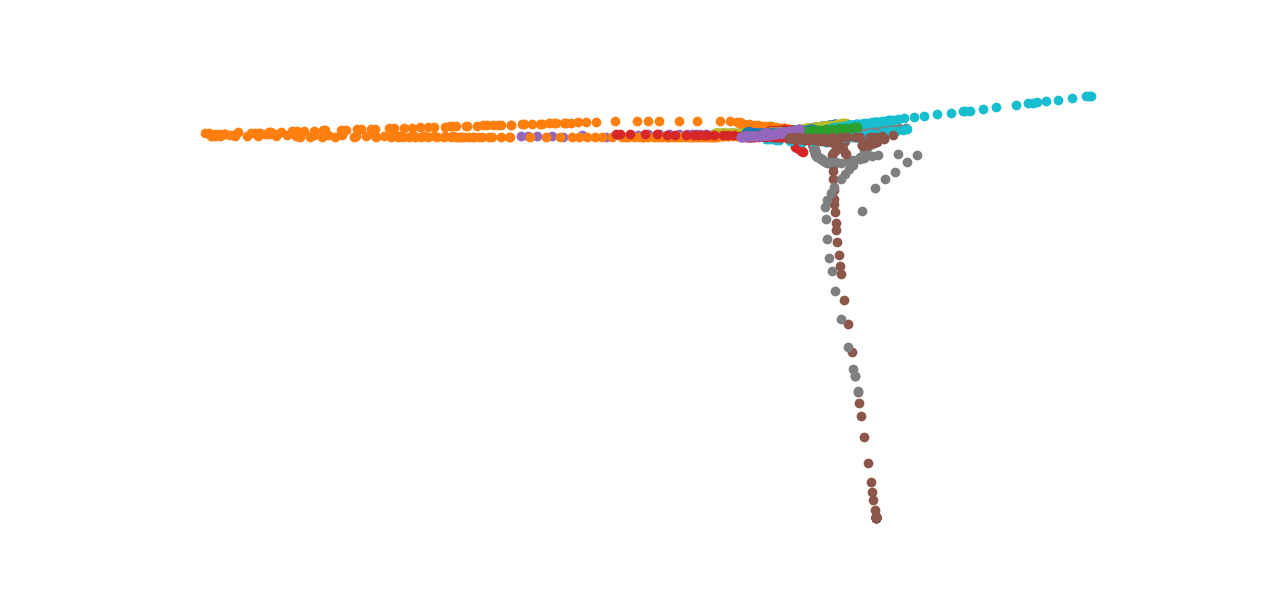
\includegraphics[width=1\textwidth]{images/dimredcomps/LLE_sins.png}\\
		  ISOMAP\\
                  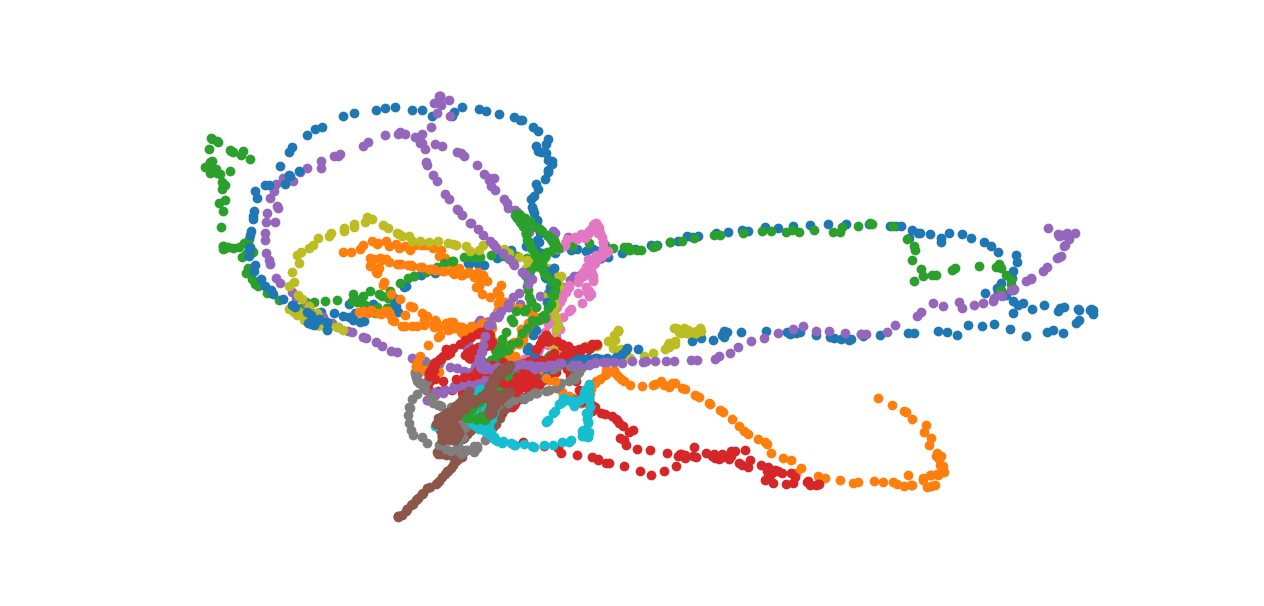
\includegraphics[width=1\textwidth]{images/dimredcomps/ISOMAP_sins.png}\\
		  \end{minipage}
			~
		  \begin{minipage}{0.47\textwidth}
	          UMAP\\
                  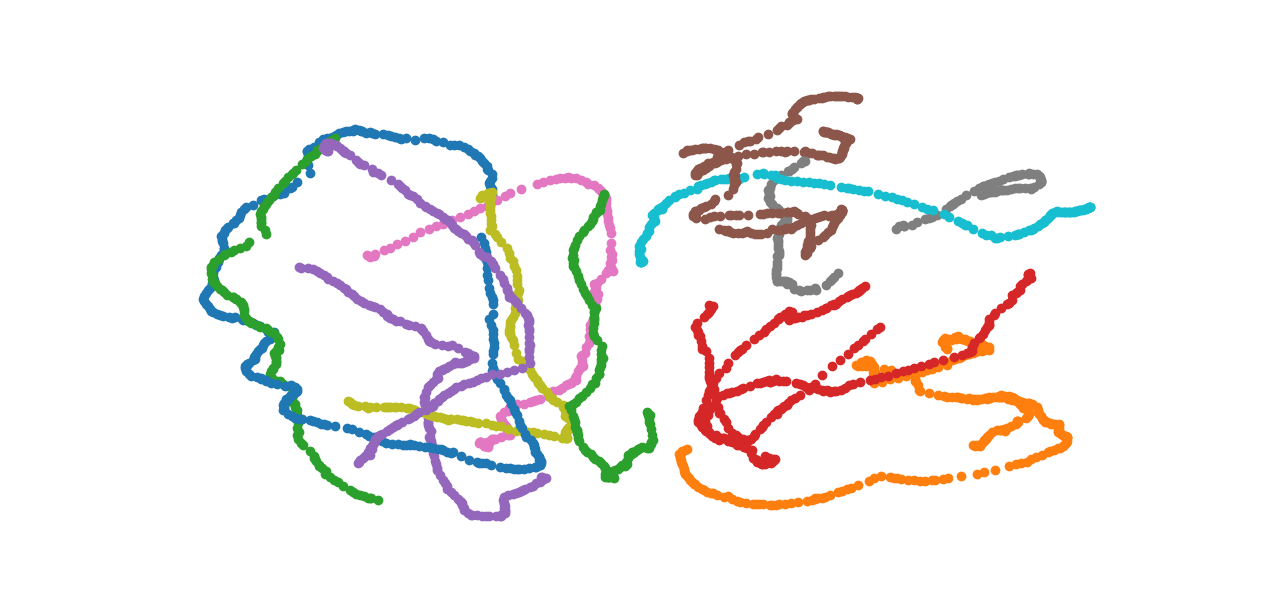
\includegraphics[width=1\textwidth]{images/dimredcomps/UMAP_sins.png}\\
		  TSNE\\
                  \includegraphics[width=1\textwidth]{images/dimredcomps/TSNE_sins.png}\\
		  \end{minipage}
	\end{center}}
        \only<2>{
	\begin{center}
		  \begin{minipage}{0.47\textwidth}
	          LLE\\
                  \includegraphics[width=1\textwidth]{images/dimredcomps/LLE_gt.png}\\
		  ISOMAP\\
                  \includegraphics[width=1\textwidth]{images/dimredcomps/ISOMAP_gt.png}\\
		  \end{minipage}
			~
		  \begin{minipage}{0.47\textwidth}
	          UMAP\\
                  \includegraphics[width=1\textwidth]{images/dimredcomps/UMAP_gt.png}\\
		  TSNE\\
                  \includegraphics[width=1\textwidth]{images/dimredcomps/TSNE_gt.png}\\
		  \end{minipage}
	\end{center}}
\end{frame}

\begin{frame}[fragile]{UMAP} 
	\begin{center}
          \vspace{-1em}
            \includegraphics[width=0.15\textwidth]{images/projSNR1.png}
            \includegraphics[width=0.15\textwidth]{images/projSNR1_2.png}
            \includegraphics[width=0.15\textwidth]{images/projSNR1_3.png}
            \includegraphics[width=0.15\textwidth]{images/projSNR1_4.png}
		  \begin{minipage}{0.47\textwidth}
	          SNR 1\\
                  \includegraphics[width=0.9\textwidth]{images/dimredcomps/UMAP_gt_snr1.png}\\
		  SNR 1/3\\
                  \includegraphics[width=0.9\textwidth]{images/dimredcomps/UMAP_gt_snr1_3.png}\\
		  \end{minipage}
			~
		  \begin{minipage}{0.47\textwidth}
	          SNR 1/2\\
                  \includegraphics[width=0.9\textwidth]{images/dimredcomps/UMAP_gt_snr1_2.png}\\
		  SNR 1/4\\
                  \includegraphics[width=0.9\textwidth]{images/dimredcomps/UMAP_gt_snr1_4.png}\\
		  \end{minipage}
	\end{center}
\end{frame}

\begin{frame}[fragile]{TSNE} 
	\begin{center}
          \vspace{-1em}
            \includegraphics[width=0.15\textwidth]{images/projSNR1.png}
            \includegraphics[width=0.15\textwidth]{images/projSNR1_2.png}
            \includegraphics[width=0.15\textwidth]{images/projSNR1_3.png}
            \includegraphics[width=0.15\textwidth]{images/projSNR1_4.png}
		  \begin{minipage}{0.47\textwidth}
	          SNR 1\\
                  \includegraphics[width=0.9\textwidth]{images/dimredcomps/TSNE_gt_snr1.png}\\
		  SNR 1/3\\
                  \includegraphics[width=0.9\textwidth]{images/dimredcomps/TSNE_gt_snr1_3.png}\\
		  \end{minipage}
			~
		  \begin{minipage}{0.47\textwidth}
	          SNR 1/2\\
                  \includegraphics[width=0.9\textwidth]{images/dimredcomps/TSNE_gt_snr1_2.png}\\
		  SNR 1/4\\
                  \includegraphics[width=0.9\textwidth]{images/dimredcomps/TSNE_gt_snr1_4.png}\\
		  \end{minipage}
	\end{center}
\end{frame}

\begin{frame}[fragile]{Flowchart}
  \begin{center}\includegraphics[width=1\textwidth]{images/second_pipeline.png}
    \end{center}
    \placetextbox[north west]{0}{0.63}{\setlength{\fboxsep}{0pt}\setlength{\fboxrule}{0.5pt}\includegraphics[width=0.7\textwidth]{images/dimredcomps/UMAP_sins.png}}

    \pause
    But how do we assign clusters?
\end{frame}

\section{Clustering}
\begin{frame}{The data}
  \includegraphics[width=0.49\textwidth]{images/figures/TSNE_raw_cyan.png}
  \pause
  \includegraphics[width=0.49\textwidth]{images/figures/TSNE_gt.png}\\
  Ground truth: Good separation between two classes - but discontinuous \\
  \pause
  We know which sinogram each line comes from... \\
  Lines from one sinogram are initial clusters

  % Figures from update page
  %% yes, we can use the relationship between single lines from the same sinogram and from the same model.
  %% Cant use conventional clustering algorithms as cluster is not all spatially in the same place.
  %% We made our own based off of agglomerative method.
  %% For 800 (400 each from two classes) we get 100 \% success in clustering. Takes 20 minutes...
  %% For 800 (200 each from 4 classes, 2 classes very similar) we get  100\% success in clustering the differnt 3.
  %% In order to know where to cut the tree we look when a large jump occurs. - Two large groups merging

  %% Issues with clustering: Ctf, off centering, noise.
\end{frame}

\begin{frame}{Heirarchical clustering}
  \begin{center}
  \begin{minipage}{0.35\textwidth}
  \includegraphics[width=1\textwidth]{images/tree_with_sins.png}
  \end{minipage}
  \begin{minipage}{0.55\textwidth}
    \begin{itemize}
        \item S1 – S5 Are Sinograms.
        \item S1 and S2 are clustered together into C1 due to good overlap.
        \item Continue clustering best scoring groups until one cluster remains containing all Sinograms.
        \item Can cut tree at any point and make models with clustered projections.
    \end{itemize}
  \end{minipage}
  \end{center}
\end{frame}

\begin{frame}[fragile]{Flowchart}
  \begin{center}\includegraphics[width=1\textwidth]{images/third_pipeline.png}
    \end{center}
    \placetextbox[north west]{0.13}{0.60}{\setlength{\fboxsep}{0pt}\setlength{\fboxrule}{0.5pt}\includegraphics[width=0.4\textwidth]{images/figures/TSNE_gt.png}}
    \pause
    \vspace{1em}\\Just a model left!
\end{frame}

\begin{frame}{Experiments}
    \begin{center}
      \begin{minipage}{0.45\textwidth}
        \includegraphics[width=1\textwidth]{images/model_tree.png}
      \end{minipage}
      \begin{minipage}{0.45\textwidth}
        \includegraphics[width=1\textwidth]{images/model_comp.png}
        \pause
        \includegraphics[width=1\textwidth]{images/exp_plots.png}
      \end{minipage}
    \end{center}
\end{frame}

%% \section{Reconstruction}

%% \begin{frame}[fragile]{Angular recovery from 3 Common lines}
%%   \textbf{Common line gives axis of rotation.}
%%   Three common lines gives 2 unique solutions for 3D orientation (One mirror of other)
%%   \only<1>{\begin{center}\includegraphics[width=0.45\textwidth]{images/Sinogram_3_comp.png}
%%     \end{center}}
%%   \only<2->{\begin{center}\includegraphics[width=0.801\textwidth]{images/vectors.png}
%%     \end{center}}
%%   \textit{\tiny{Angular Reconstitution: A Posteriori Assignment of Projection Directions for 3d Reconstruction. Van Heel 1987}}
%%   \only<3>{\placetextbox[north west]{0.34}{0.63}{\includegraphics[width=0.4\linewidth]{images/3_line_model.png}}}
%% \end{frame}

%% \begin{frame}[fragile]{Eigenvector Relaxation}
%%   \small
%%   \textbf{Aim: Given all common lines $c$ for projections $P$, assign Rotation matrices $R$ for each $P$ to give greatest consensus volume.}
%%   \begin{center}
%%     \begin{minipage}{0.45\textwidth}
%%         \includegraphics[width=\textwidth]{images/radon_ft.png}
%%         Maths*! Make large $(2N \times 2N)$ symmetric matrix $S$. Can recover $R$ for each $P$ from top 3 eigenvalues of $S$ that maximise consistency function!
%%     \end{minipage}
%%     ~~~
%%     \begin{minipage}{0.45\textwidth}
%%       %% \tiny{$$cij~=~(cos(\theta_{ij}),sin(\theta_{ij}),0),$$\\$$~cji~=~(cos(\theta_{ji}),sin(\theta_{ji}),0)~\quad~(1)$$}
%%       %%   $$max\sum_{i\ne j} R_ic_{ij} \cdot R_jc_{ji} \quad (2)$$
%%         \includegraphics[width=\textwidth]{images/eighist.png}
%%     \end{minipage}

%%   \end{center}

%%   \vspace{2em}
%%   \textit{\scalebox{0.5}{*Three Dimensional Structure Determination from Common Lines in Cryo-EM by Eigenvectors and Semidefinite Programming. A.Singer and Y.Shkolnisky}}
%% \end{frame}

\begin{frame}{Any Questions?}
    \begin{center}
      \begin{minipage}{0.45\textwidth}
        Thanks to eBIC, \\
        Yuriy Chaban - The Concept \\
        \& \\
        CCPEM \\
      \end{minipage}
      \begin{minipage}{0.45\textwidth}
        \begin{center}
          \includegraphics[height=0.4\textheight]{images/proj_sin_lin.png}
          \includegraphics[height=0.4\textheight]{images/UMAP_heart.png}
        \end{center}
      \end{minipage}
    \end{center}
\end{frame}


\end{document}

%% \section{Reconstruction}
%% \subsection*{Too many Lines}
%% % \begin{frame}[fragile]{Voting}
%% %   Take all lines pairs under distance X
%% %   This gives multiple possible axis between the same two projections. Weight these according to distance and number of times they appear.
%% %   For each common line between two sinograms get more than 1 match so... vote which is best!
%% % \end{frame}

%% % \begin{frame}[fragile]{Overdetermined system}
%% %   % https://www.osapublishing.org/josaa/fulltext.cfm?uri=josaa-9-10-1749&id=64057
%% %   3 projections can satisfy geometrical constraints.
%% %   Problem when we add a fourth!
%% %   R = matrix
%% %   need 6 variables per projection.
%% %   Each pair of projection gives us 2 variables. 
%% %   2 N^2 vs 6N
%% %   if N = 3 then we have determined system
%% %   3 lines is all good for getting angular information back c.f. prev slide.
%% %   any more than 3 and we can get contradicting equations - system is overdetermined. we have N\^2 linear equations and only 6N variables (do proper maths)
%% %   Machine learning 3! how to fit. Least squares optimization not good as we have large number of misidentified lines and nonconvex! we also need to get proper rotation matrices at the end. This constraint leads to collapse to trivial solution 000. Need other approach.
%% % \end{frame}

